\section*{Question II}

\begin{figure}[H]
\centering
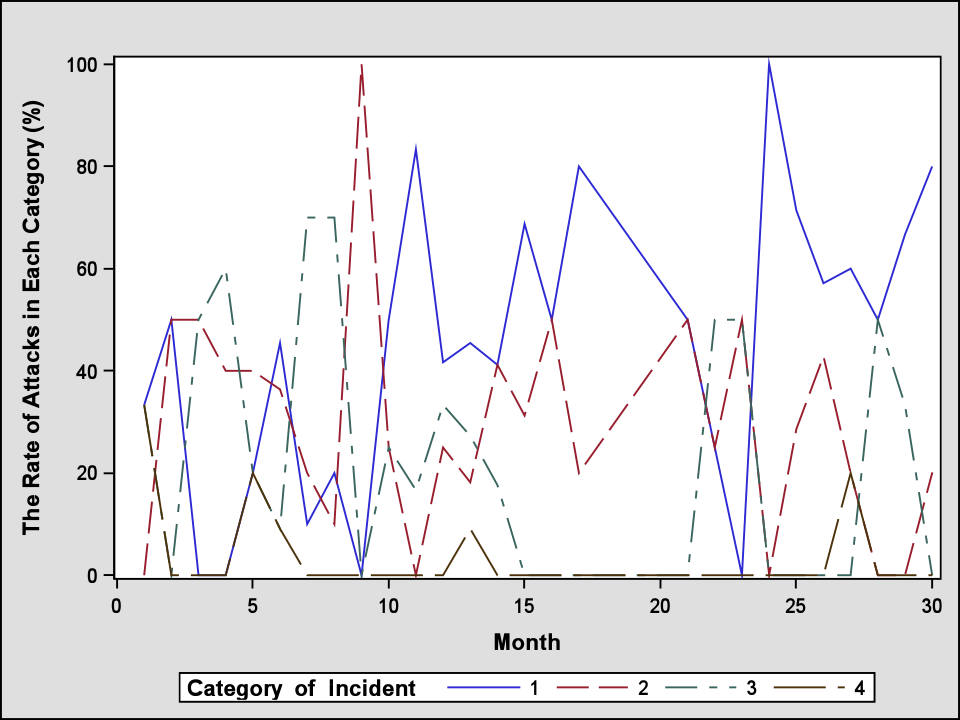
\includegraphics[scale=0.25]{Pic/Q2/1.png}
\caption{The Rate of Attacks in Each Category}
\label{f5}
\end{figure}

At the outset, we can see that it is not the same throughout the 30-month period by the figure \ref{f5} above.

\begin{figure}[htbp]
\centering
\begin{minipage}[t]{0.48\textwidth}
\centering
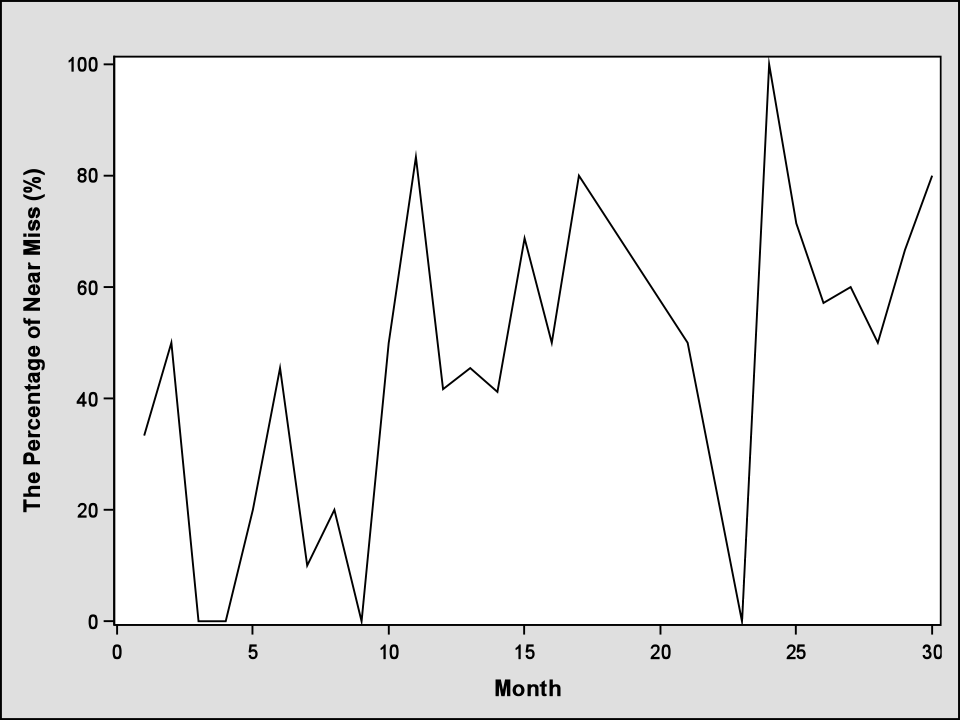
\includegraphics[width=6cm]{Pic/Q2/2.png}
\caption{The Percentage of Near Miss}
\label{f6}
\end{minipage}
\begin{minipage}[t]{0.48\textwidth}
\centering
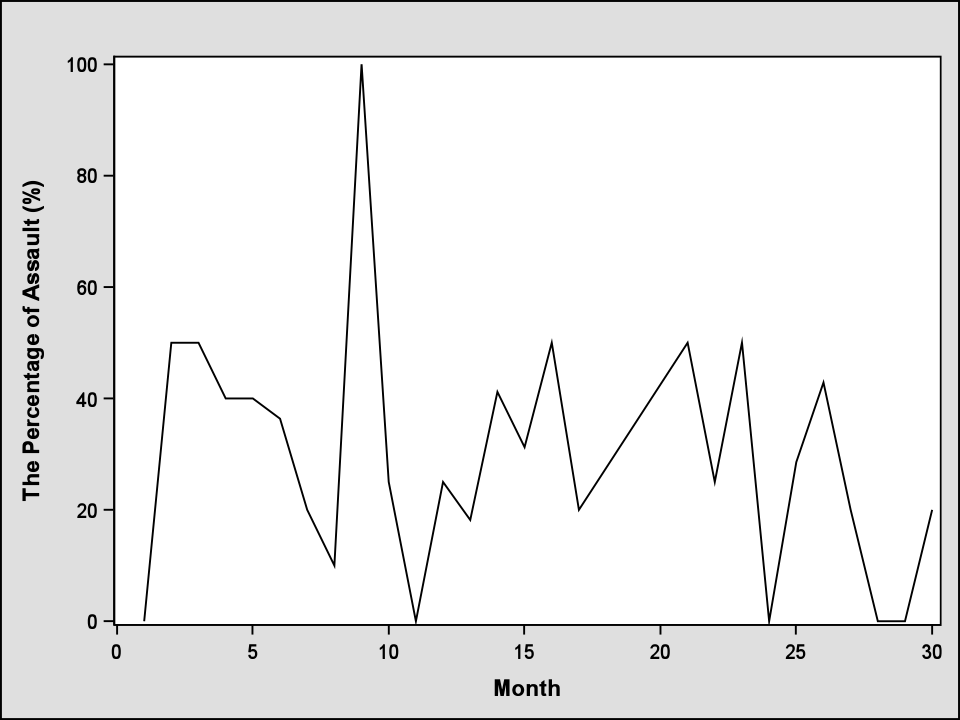
\includegraphics[width=6cm]{Pic/Q2/3.png}
\caption{The Percentage of Assault}
\label{f7}
\end{minipage}
\end{figure}

Moreover, these two figures (\ref{f6}, \ref{f7}) show that is not always
proportional to the number of attacks each month.

\begin{figure}[H]
\centering
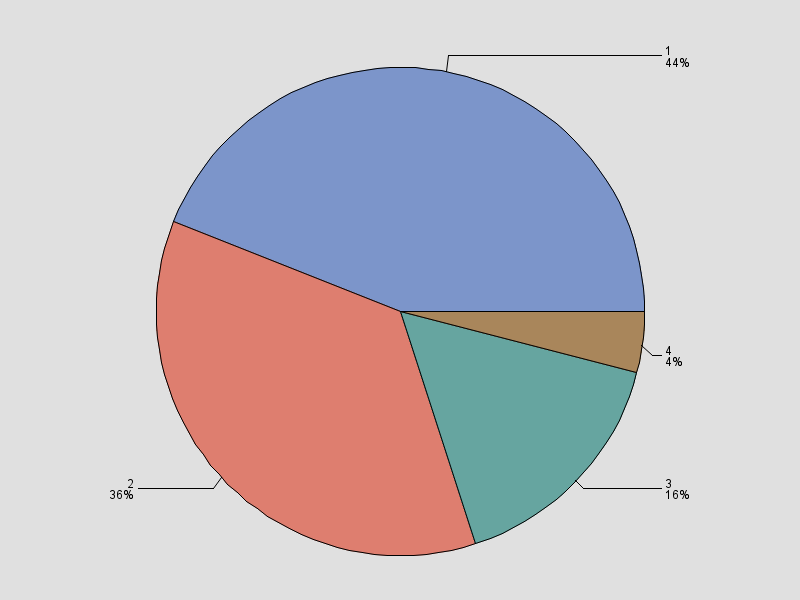
\includegraphics[scale=0.5]{Pic/Q2/4.png}
\caption{The Rate of Attacks in Each Category for the Second Half
of the 30 Months}
\label{f8}
\end{figure}
Finally, figure (\ref{f8}) shows that there was a higher proportion of less threatening incidents in the second half
of the 30 months. In conclusion, these figures demonstrate the fact that less threatening incidents accounts a higher proportion. The option B may be the correct answer.
